
\documentclass[12pt]{article}
\usepackage[paper=letterpaper,margin=2cm]{geometry}

\usepackage{amsmath}
\usepackage{amsthm} %needed for the proofs 
\usepackage{amssymb}
\usepackage{titling}
\usepackage{thmtools}
\usepackage{mathptmx} %font
\usepackage{verbatim} % for comments
\usepackage{mdframed}
\usepackage[linesnumbered,ruled,vlined]{algorithm2e}
\usepackage{lipsum}

\usepackage[T1]{fontenc} %header
\usepackage[utf8]{inputenc}%header
\usepackage{geometry} %header
\usepackage{fancyhdr}%header

\usepackage{forest} % for decision trees

%images
\usepackage{graphicx}
\graphicspath{ {./images/} }
% to include an image, do: 
%    \begin{center}
%    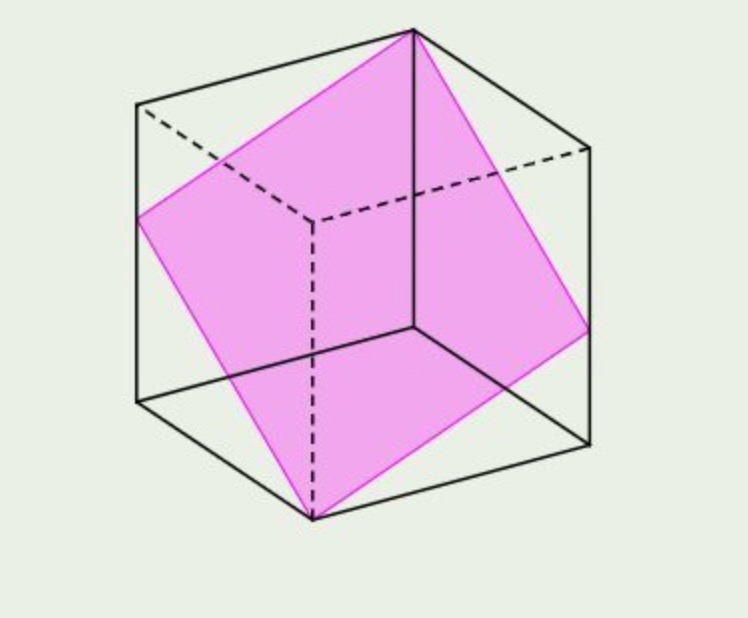
\includegraphics[scale=0.20]{graph.jpg}
%    \end{center}
% OR: 
%\begin{figure}
%    \centering
%    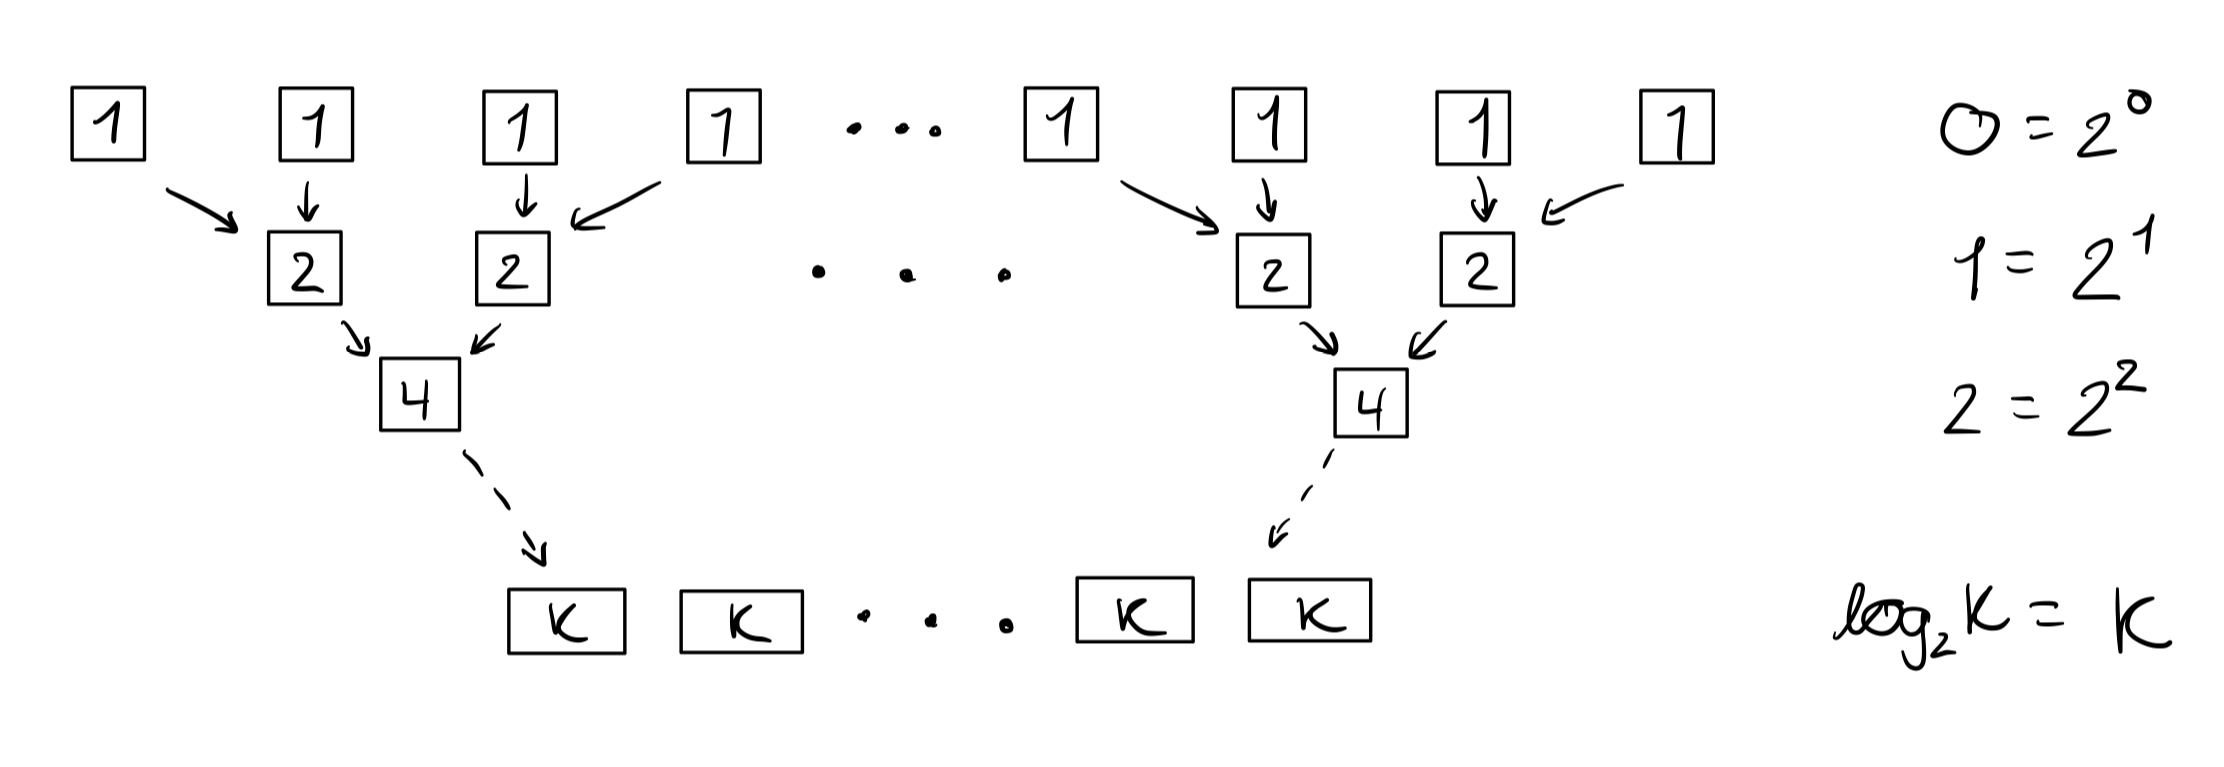
\includegraphics[scale=0.20]{IMG_1052.jpg}
%    \caption{Your caption text here.}
%\end{figure}


%macros for recursive functions
%For plots
\usepackage{pgfplots}
\pgfplotsset{compat = newest}

\newtheorem{theorem}{Theorem}
\declaretheoremstyle{lemma}
\declaretheorem[style=lemma, name=Lemma]{lemma}

\theoremstyle{definition}
\newtheorem{definition}{Definition}

\declaretheoremstyle{example}
\declaretheorem[style=example, name=Example]{example}

\theoremstyle{remark}
\newtheorem*{remark}{Remark}

\declaretheoremstyle{proposition}
\declaretheorem[style=proposition, name=Proposition]{proposition}

\declaretheorem[name=Note]{note}
\declaretheoremstyle{note}

\setlength\parindent{24pt}%set paragraph indent

\newenvironment{ftheo}
  {\begin{mdframed}\begin{theorem}}
  {\end{theorem}\end{mdframed}}


  % --- Special commands --- %
\newcommand\sol{%
  \\ 
  \\
  \textit{Solution:}\\%
}
% Statistics
\newcommand{\indep}{\perp \!\!\! \perp}
\DeclareMathOperator{\var}{Var}
\DeclareMathOperator{\cov}{Cov}

%Convex optimisation operators
\DeclareMathOperator{\cl}{cl}
\DeclareMathOperator{\epi}{epi}
\DeclareMathOperator{\lev}{lev}
\DeclareMathOperator{\dom}{dom}
\DeclareMathOperator{\aff}{aff}
\DeclareMathOperator{\ri}{ri}
\DeclareMathOperator{\argmin}{argmin}

% --- Header --- %
\renewcommand{\headrulewidth}{.4mm} % header line width

\pagestyle{fancy}
\fancyhf{}
\fancyhfoffset[L]{1cm} % left extra length
\fancyhfoffset[R]{1cm} % right extra length
\rhead{\today}
\lhead{\it Alexandre St-Aubin \& Dylan Telio}
\rfoot{}

% --- Title Page --- % 
\setlength{\droptitle}{-6em}

\title{\textsc{Assignment 3 -- COMP 252}}  
\author{\it Alexandre St-Aubin and Dylan Telio}
\date{\today}

\begin{document}
\maketitle 
\begin{enumerate}
  \item \textsc{Decision tree lower bound.}
  \begin{enumerate}
    \item[\it (i)]Give a simple algorithm for this problem and an upper bound on the complexity. For n = 5, your answer should be 7.
    \sol
    \begin{algorithm}
    \caption{An algorithm to classify the $n$ monkeys. }
    \SetKwRepeat{Do}{do}{while} %do-while loop macro
    \SetKwInput{KwOut}{Output}
    \SetKwInput{KwIn}{Input}
    \SetKwData{monk}{Monkeys}
      \SetKwData{app}{append}
    \SetKwData{typea}{Species\_1}
    \SetKwData{typeb}{Species\_2}
    \SetKwData{typec}{Species\_3}
    \KwIn{An array \monk of monkeys.}
    \KwOut{Three arrays separating the monkey species.}
    \BlankLine
    \typea $\leftarrow$ new Array;  \\ 
    \typeb $\leftarrow$ new Array;  \\ 
    \typec $\leftarrow$ new Array;  \\ 
    $i \leftarrow 1;$\\ 
    $\typea.\app(\monk[0])$;\\
      \While{$\monk[0] = \monk[i]$}{
        $\typea.\app(\monk[i])$; \\ 
        $i++;$\\ 
      }
      \tcp{loop above exits only if a second monkey species was found}
      $\typeb.\app (\monk[i]);$
    \BlankLine 
      \tcp{for each remaining monkey, compare to the 2 known species}
      \For{$j$ in range $[i, n]$ }{
      \If{$\monk[j] = \typea[0]$}{
      \typea.\app(\monk[j]);
      }\ElseIf{$\monk[j] = \typeb[0]$}{
      \typeb.\app(\monk[j]);
      }\Else{
      \typec.\app(\monk[j]);
      }
      }
  \end{algorithm}
    \begin{remark} 
      The worst case for the above algorithm is when the two first monkeys are different, and each remaining monkey is of the third or second species, hence must be compared twice (once to each of the first two species), in order to be classified. This yields an upper bound complexity of $1 + 2(n-2).$ When $n = 5, $ this is indeed equal to 7.
    \end{remark} 
    \newpage
    \item[\it (ii)] Show that all leaves in the decision tree must be different (i.e., correspond to different outputs).
\begin{proof} 
    Fix a sequence of monkeys. The decision tree representing the algorithm described in part $(i)$ is binary, where each decision takes as input two monkeys, and outputs whether they are of the same species or not. Every monkey must be compared at most twice to be classified. We can represent each comparison by a bit, 1 being a match, and 0 otherwise. The output for a given monkey will therefore be: 
   $$\left\{ \begin{matrix}
     10 & \text{ if match with Species\_1} \\ 
01 & \text{ if match with Species\_2} \\ 
00 & \text{ if match with Species\_3} 
   \end{matrix} \right.$$
    We note that in reality, if there is a match with Species\_1, the monkey will not be compared with the other species, as it would be useless. So, the notation $10$ is not entirely representative of what truly happens in the algorithm, it should rather be $1$, as only one comparison is made. However, for sake of notation, we keep it as $10.$

    \hspace{24pt}Hence, one easily sees that each leaf in the decision tree can be represented as a binary sequence of comparisons, where each 2 consecutive bits represents the classification of a monkey. In order to relax notation, let $10 = 1, \; 01 = 2,\; 00 = 3 $, then each leaf is given as a sequence of the form
    $$1233322123123121$$
    We show by induction that each leaf represents a unique monkey sequence. The base case is clear when $n =2$. Now, assume that for $n-1$ monkeys, each leaf is represented by a unique sequence of the numbers $\{1,2,3\}$ of length $n-1$. Then, if we add a monkey to the end of the array of monkeys, for each existing sequence $\{a_i\}_{i=1}^{n-1}$, 3 sequences of length $n$ will be created: 
    $$a_{i,1} := \{a_i\}_{i=1}^{n-1}\cup \{a_n = 1\}  $$
  $$a_{i,2} := \{a_i\}_{i=1}^{n-1}\cup \{a_n = 2\}  $$
  $$a_{i,3} := \{a_i\}_{i=1}^{n-1}\cup \{a_n = 3\}  $$

  Clearly the 3 new sequences are unique for each $i$, and since the $n-1$ first elements of every sequence are unique by the induction hypothesis, it follows that all of the sequences representing the decision tree for $n$ monkeys are unique. Hence, the leaves represent unique outputs. 

\end{proof}
     \item[\it (iii)] Using a decision tree-based method, show that the lower bound for this problem is 6 when $n = 5$.
     \begin{proof} 
      The algorithm outputs three sets of monkeys of identical species. For each monkey, there are three possibilities of species, hence $3^5$ total permutations. Yet, this accounts for the order of the species, which we don't care about. That is, it shouldn't matter whether the \textit{popa langurs} are grouped in Species\_1, Species\_2, or Species\_3. To remove this unwanted notion of order, we divide by $3!$. It follows that the total number of possible outputs of the algorithm is given by
    $$\frac{3^n}{3!} $$
       By part (ii), each leaf corresponds to a different output, so we have a tree with $\frac{3^n}{3!}$ leaves. Thus, by the method of decision trees, the lower bound is
    $$\left\lceil\log_{2}\left( \frac{3^5}{3!} \right)\right\rceil = 6$$

     \end{proof}
  \item[\it (iv)] For general $n,$ show that the decision tree lower bound is at least $an- b$ and at most $an + b$
    for $n \geq n_0$, for some positive numbers $a, b, n_0$. Determine suitable values for these numbers. Compare this with your answer in \textit{(i)} and conclude that the decision tree bound for this problem is rather weak.
  \end{enumerate}
  \newpage
  \item \textsc{Adversarial lower bound.} Using the method of adversaries, show that the lower bound for this problem is 7 when $n = 5$. 
  \sol 
  \textsc{Adversary Strategy:} The adversary always answers NO, unless it has to answer YES.

  \textbf{Claim}: This strategy always yields at least 7 comparisons.
  \begin{proof} 
    Denote the set of monkeys by $\Omega := \{a,b, c,d,e\}$. There are two cases where the adversary must answer "yes" to a comparison between two monkeys. Without loss of generality, let $a \in $ Species\_1 and $x\in \Omega$, then the adversary will be forced to answer yes if,
    \begin{enumerate}
      \item[\it (i)] $x$ was already compared to Species\_2 and Species\_3, and the adversary answered "no" to both.
      \item[\it (ii)] $x$ was already compared to Species\_1 and the adversary answered "yes". 
    \end{enumerate}
    Notice that in either case, the algorithm doesn't gain any new information. We may therefore assume that the adversary will never be forced to answer "yes", as any good algorithm would not waste comparisons to obtain information it already knows. 
  \end{proof}


  \newpage
  \item \textsc{Lower bounds by the method of adversaries, and an algorithm.}

\end{enumerate}
\end{document}
